\documentclass[dvipdfmx]{beamer}
\usepackage{bxdpx-beamer}% dvipdfmxなので必要
\usepackage{pxjahyper}% 日本語で'しおり'したい
%\usepackage{etex}
%\usetheme{Warsaw}
\usetheme{Malmoe}
%\usetheme{AnnArbor}
%\usetheme{Hannover}
%\usetheme{Bergen}
%\usetheme{Berlin}
%\usetheme{Singapore}
%\usetheme{Montpellier}
%\usetheme{Pittsburgh}
\usepackage{graphicx}
\usepackage{latexsym,amssymb}
%\usepackage{epsbox}
%\usepackage{multirow}
\usepackage{fancybox}
\usepackage{fancyvrb}
%\usepackage{listings}
\usepackage{tabularx}
\usepackage{tikz}
\usetikzlibrary{calc,shapes}
%\usepackage{pstricks,pst-node,pst-tree}
%\usepackage{multimedia}
%\usepackage{pstricks,pst-node,pst-tree}
%\usepackage{pst-all}
%\include{prooftree}
%\lstloadlanguages{pascal}
\renewcommand{\kanjifamilydefault}{\gtdefault}
\renewcommand{\familydefault}{\sfdefault}

%\include{cmacros}

\graphicspath{{fig251107/}}

\newcommand{\greentext}[1]{{\color[rgb]{0,0.5,0}{#1}}}
\newcommand{\redtext}[1]{{\color[rgb]{0.8,0,0}{#1}}}
\newcommand{\bluetext}[1]{{\color[rgb]{0,0,0.8}{#1}}}

\newcommand{\tuple}[1]{\langle{#1}\rangle}

\newcommand{\First}{\mathsf{First}_1}
\newcommand{\Follow}{\mathsf{Follow}_1}

%%pdt simulation

\newcommand{\pdtline}[6]{%
    \uncover<#6->{
    \node at (${#5}*(0,-.3)+(0,.3)$) {$\vdash$};%
    \node at (${#5}*(0,-.3)+(1.5,.3)$) {\parbox{12em}{(#1,}};%
    \node at (${#5}*(0,-.3)+(4.5,.3)$) {\parbox{10em}{#2,}};%
    \node at (${#5}*(0,-.3)+(5.7,.3)$) {\parbox{10em}{#3)}};%
    \node at (${#5}*(0,-.3)+(8,.3)$) {\parbox{20em}{#4}};%
    }
}

\newcommand{\initpdtline}[6]{%
    \uncover<#6->{
    \node at (${#5}*(0,-.3)+(1.5,.3)$) {\parbox{12em}{(#1,}};%
    \node at (${#5}*(0,-.3)+(4.5,.3)$) {\parbox{10em}{#2,}};%
    \node at (${#5}*(0,-.3)+(5.7,.3)$) {\parbox{10em}{#3)}};%
    \node at (${#5}*(0,-.3)+(8,.3)$) {\parbox{20em}{#4}};%
    }
}

\newtheorem{Def}{定義}
\newtheorem{Lem}{補題}
\newtheorem{Thm}{定理}
\newtheorem{Prop}{命題}

\definecolor{lightlightgrey}{rgb}{0.95,0.95,0.95}



%\newcommand{\greentext}[1]{{\color[rgb]{0,0.5,0}{#1}}}
%\newcommand{\redtext}[1]{{\color[rgb]{0.8,0,0}{#1}}}

\newcommand{\lecturedate}{2025/11/7}

\cornersize{0.25}

\setbeamertemplate{frametitle}[default][center]
\setbeamertemplate{footline}{\hfill
コンパイラ\quad\lecturedate
\hfill\insertframenumber/\inserttotalframenumber\hspace*{1zw}}
\newcounter{coffee}
\setbeamercovered{transparent=10}
\title{コンパイラ(11)}
\date{\lecturedate}
\begin{document}

\frame{\titlepage}

\section{構文主導型変換}

\subsection{属性文法}

\begin{frame}
 \frametitle{属性文法}

 属性文法(attribute grammar):抽象構文木に属性を加えた文法

 \greentext{構文主導型変換への応用=コード生成に関する情報を属
 性として扱う}

 属性文法 $A_g=(G,{\cal A},E)$
 \begin{list}{}{}
  \item $G=(N,\Sigma,P,S)$はCF文法
  \item ${\cal A}$:属性の集合\\
	${\cal A}=\cup_{X\in
	N\cup\Sigma}{\cal A}(X)$.  $a\in{\cal A}(X)$のとき、
	$X.a$と書く。
  \item $E$:意味規則の集合\\
	$p\in P$に対して以下のような規則定める。
	\[
	 p\{X_i.a_i=f_i(X_{i_1}.a_{i_1},\ldots,X_{i_n}.a_{i_n})\}
	\]
 \end{list}

 \[\begin{array}{ll}
  E\rightarrow E^{(1)}\texttt{+}E^{(2)} & \{E.val=E^{(1)}.val+E^{(2)}.val\}\\
  E\rightarrow \texttt{NUM} & \{E.val=\texttt{NUM}.val\}
 \end{array}
   \]
%  \begin{center}
%   \includegraphics[scale=1]{figs191113/attribGram01.eps}
%  \end{center}

\end{frame}


\begin{frame}
 \frametitle{属性の種類}

 \begin{list}{}{}
  \item 合成(synthesized)属性\\
	\greentext{右辺の属性から合成された左辺の属性}:
  \item 相続(inherited)属性 (「継承属性」とも言う)\\
	\greentext{合成以外の属性}
 \end{list}


 \[G=(\{T,L\},\{\texttt{MAX},\texttt{MIN},\texttt{NUM},`\texttt{(}',`\texttt{)}',`\texttt{,}'\},P,T)\]

 \scalebox{0.8}{
 $\mathcal{A}$:
 \begin{tabular}{|c|c|c|}\hline
    & 合成属性 & 相続属性\\\hline
  $T$ & $T.val$ & \\\hline
  $L$ & $L.val$ & $L.op$\\\hline
 \end{tabular}
 }

\vspace*{5pt}

{\small
%P,E:\\

$P=\left\{\begin{array}{ll}
  T\rightarrow\texttt{MIN'('}L\texttt{')'} & \{L.op=\texttt{MIN},T.val=L.val\}\\
  T\rightarrow\texttt{MAX'('}L\texttt{')'} & \{L.op=\texttt{MAX},T.val=L.val\}\\
  L\rightarrow\texttt{NUM} & \{L.val=\texttt{NUM}.val\}\\
  L\rightarrow L^{(1)}\texttt{',' NUM} & \left\{\begin{array}{l}L.val=f(L.op,L^{(1)}.val,\texttt{NUM}.val),\\
    L^{(1)}.op=L.op\end{array}\right\}
\end{array}\right\}$
 }
%  \begin{center}
%   \includegraphics[scale=.8]{figs191113/AttributeExample.eps}
%  \end{center}
\end{frame}

\begin{frame}
  \frametitle{属性文法に基づくコード生成例}
  $G$に生成規則$\{S\rightarrow T\#\}$を加えた拡張文法に対するLR解析

  \vspace*{3pt}

  $P=\left\{\begin{array}{rlcrl}
    0: & S\rightarrow T\#, & & 3: & L\rightarrow\texttt{NUM},\\
    1: & T\rightarrow\texttt{MIN}\ `\texttt{(}'\ L\ `\texttt{)}', & & 4: & L\rightarrow L\ `\texttt{,}'\ \texttt{NUM},\\
    2: & T\rightarrow\texttt{MAX}\ `\texttt{(}'\ L\ `\texttt{)}' & & & 
  \end{array}\right\}$

  \vspace*{3pt}

  $\mathsf{Follow}_1(T)=\{\#\}$, 
  $\mathsf{Follow}_1(L)=\{\texttt{)},`\texttt{,}'\}$


\end{frame}

\begin{frame}
  \frametitle{属性文法に基づくコード生成例}
  \begin{center}
  \begin{tabularx}{\textwidth}{XX}
  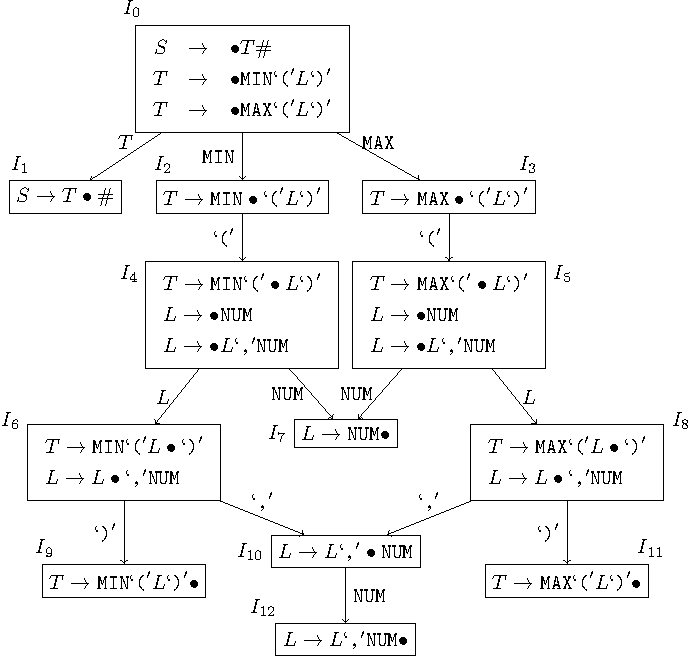
\includegraphics[scale=0.45]{maxmin-lrautomaton-crop.pdf}
  &
  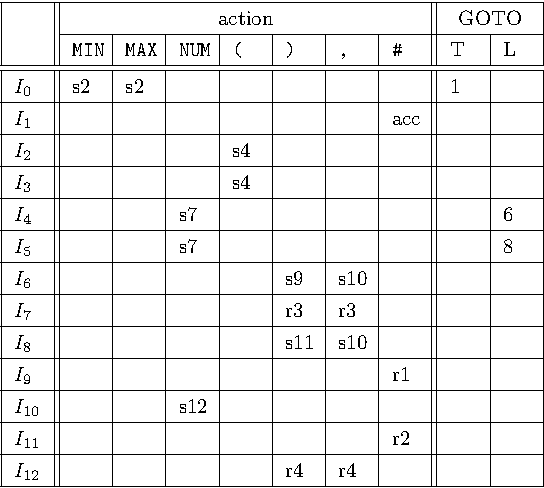
\includegraphics[scale=0.5]{maxmin-parsetab-crop.pdf}\\
  {\small LR(0)遷移系} & {\small SLR(1)構文解析表}
  \end{tabularx}
\end{center}
\end{frame}

\begin{frame}
  \frametitle{属性文法に基づくコード生成例}
  \scriptsize{
  \[
    \begin{array}{clllll}
       & (I_0,& \texttt{MIN(3,5,7)\#},& \varepsilon)\\
    \vdash & (I_0\texttt{MIN}I_2, & \texttt{(3,5,7)\#},& \varepsilon)\\
    \vdash & (I_0\texttt{MIN}I_2\texttt{(}I_4, & \texttt{3,5,7)\#}, & \varepsilon)\\
    \vdash & (I_0\texttt{MIN}I_2\texttt{(}I_4\texttt{3}I_7, & \texttt{,5,7)\#}, & \varepsilon)\\
    \vdash & (I_0\texttt{MIN}I_2\texttt{(}I_4 L I_6, & \texttt{,5,7)\#},& 3) & \%1.val=3\\
    \vdash & (I_0\texttt{MIN}I_2\texttt{(}I_4 L I_6\texttt{,}I_{10}, & \texttt{5,7)\#},& 3)\\
    \vdash & (I_0\texttt{MIN}I_2\texttt{(}I_4 L I_6\texttt{,}I_{10}5I_{12}, & \texttt{,7)\#}, & 3)\\
    \vdash & (I_0\texttt{MIN}I_2\texttt{(}I_4 L I_6, & \texttt{,7)\#},& 34)& \%2.val=f(\only<1>{\%1.op}\only<2>{\redtext{min}},\%1.val,5);\\
    \only<1>{       &                                         &                &    & \%2.op=\%1.op\\}
    \vdash & (I_0\texttt{MIN}I_2\texttt{(}I_4 L I_6\texttt{,}I_{10}, & \texttt{7)\#},& 34)\\
    \vdash & (I_0\texttt{MIN}I_2\texttt{(}I_4 L I_6\texttt{,}I_{10}7I_{12}, & \texttt{)\#}, & 34)\\
    \vdash & (I_0\texttt{MIN}I_2\texttt{(}I_4 L I_6, & \texttt{)\#}, & 344) & \%3.val=f(\only<1>{\%2.op}\only<2>{\redtext{min}},\%2.val,7);\\
    \only<1>{       &                                         &               &      & \%3.op=\%2.op\\}
    \vdash & (I_0\texttt{MIN}I_2\texttt{(}I_4 L I_6\texttt{)}I_9, & \texttt{\#}, & 344)\\
    \vdash & (I_0 T I_1, & \texttt{\#}, & 3441) & \only<1>{\redtext{\%3.op=min;}}\%4.val=\%3.val\\
    \vdash & (acc, & \texttt{\#}, & 34410)
    \end{array}
    \]
    }
    \only<1>{\greentext{相続属性($f$の第一引数)が最後に決定される}}
    \only<2>{\greentext{相続属性($f$の第一引数)をバックパッチによって関数を書き換える}}

    $T.val=\%4.val$
\end{frame}

\begin{frame}
  \frametitle{属性文法に基づくコード生成例}
  \scriptsize{
  \[
    \begin{array}{clllll}
       & (I_0,& \texttt{MAX(3,5,7)\#},& \varepsilon)\\
    \vdash & (I_0\texttt{MAX}I_2, & \texttt{(3,5,7)\#},& \varepsilon)\\
    \vdash & (I_0\texttt{MAX}I_2\texttt{(}I_4, & \texttt{3,5,7)\#}, & \varepsilon)\\
    \vdash & (I_0\texttt{MAX}I_2\texttt{(}I_4\texttt{3}I_7, & \texttt{,5,7)\#}, & \varepsilon)\\
    \vdash & (I_0\texttt{MAX}I_2\texttt{(}I_4 L I_6, & \texttt{,5,7)\#},& 3) & \%1.val=3\\
    \vdash & (I_0\texttt{MAX}I_2\texttt{(}I_4 L I_6\texttt{,}I_{10}, & \texttt{5,7)\#},& 3)\\
    \vdash & (I_0\texttt{MAX}I_2\texttt{(}I_4 L I_6\texttt{,}I_{10}5I_{12}, & \texttt{,7)\#}, & 3)\\
    \vdash & (I_0\texttt{MAX}I_2\texttt{(}I_4 L I_6, & \texttt{,7)\#},& 34)& \%2.val=f(\only<1>{\%1.op}\only<2>{\greentext{max}},\%1.val,5);\\
    \only<1>{       &                                         &                &    & \%1.op=\%2.op\\}
    \vdash & (I_0\texttt{MAX}I_2\texttt{(}I_4 L I_6\texttt{,}I_{10}, & \texttt{7)\#},& 34)\\
    \vdash & (I_0\texttt{MAX}I_2\texttt{(}I_4 L I_6\texttt{,}I_{10}7I_{12}, & \texttt{)\#}, & 34)\\
    \vdash & (I_0\texttt{MAX}I_2\texttt{(}I_4 L I_6, & \texttt{)\#}, & 344) & \%3.val=f(\only<1>{\%2.op}\only<2>{\greentext{max}},\%2.val,7);\\
    \only<1>{       &                                         &               &      & \%2.op=\%3.op\\}
    \vdash & (I_0\texttt{MAX}I_2\texttt{(}I_4 L I_6\texttt{)}I_9, & \texttt{\#}, & 344)\\
    \vdash & (I_0 T I_1, & \texttt{\#}, & 3442) & \only<1>{\redtext{\%3.op=max;}}\%4.val=\%3.val\\
    \vdash & (acc, & \texttt{\#}, & 34410)
    \end{array}
    \]
    }

    \only<1>{\greentext{相続属性($f$の第一引数)が最後に決定される}}
    \only<2>{\greentext{相続属性($f$の第一引数)をバックパッチによって関数を書き換える}}

    $T.val=\%4.val$

\end{frame}

% \subsection{バックパッチ}

% \begin{frame}
%  \frametitle{バックパッチ}

%  条件分岐のコード生成の場合、ラベルの値はあとで決定する

%  \[
% p  \mathsf{if}\ E\ \mathsf{then}\ S
%  \]

% \begin{center}
%  \begin{tabular}{lrl}
% 1:&    & $E$のコード\\
% 2:&    & if not $E.\mathsf{result}$ goto $L$\\
% 3:&    & $S$のコード\\
% 4:&$L$:&
%  \end{tabular}
% \end{center}

%  $S$をコンパイルするまで$L$の値は決まらない。2の時点で$L$の具
%  体的なアドレスはわからない。

% % 厳密には1パスでコード生成はできない。

% \begin{list}%
%  {$\bullet$} %default label
%  {} %formatting parameter
%  \item とび先のアドレスの表を作成しておいて、アドレスが決定した時点で
%  $L$の値を待つコードをかきかえる。 
%  \item 命令を一旦生成するがどこが未決かを管理する。
% \end{list}

% \greentext{LLVM 実行系においては，LLVM抽象マシンがラベルを解決してくれる．}

% \end{frame}



\begin{frame}{LLVMによる条件文コード}
	
	\texttt{if} {$B$} \texttt{then} {$S_1$} \texttt{else} {$S_2$}

	\vspace*{5mm}

	\begin{tabular}{l}
		\texttt{\%1 = } [$B$ を計算するコード]\\
		\texttt{br i1 \%1, label \%L1, label \%L2}\\
		\texttt{L1:}\\
    \quad [$S_1$のコード]\\
		\texttt{br label \%L3}\\
		\texttt{L2:}\\
		\quad [$S_2$のコード]\\
		\texttt{br label \%L3}\\
		\texttt{L3:}
	\end{tabular}
	
\greentext{\texttt{L1},\texttt{L2},\texttt{L3}は実際に定義される前に参照される．}

\greentext{$S_2$の後の\%3へのジャンプは不要．}

\end{frame}

\begin{frame}[fragile]
 \frametitle{条件文における論理式}
 条件文における条件の評価：結果待ち / 短絡型\\
 \greentext{条件が副作用を持つ場合に違いが出る}\\
 \texttt{if (x>100 \&\& (z=y)<30) \{ 文1 \} else \{ 文2 \}}\\
 \texttt{z=y}の評価結果は\texttt{y}の値\\
 \greentext{{\tt z=y}が実行されるか？}\\
 結果待ち=評価される、短絡型=\texttt{x>100}のとき評価される\\

\begin{tabular}{ll}
短絡型：& 条件文の評価中にif文を評価する．\\
結果待：& 条件文の式を評価してからifを評価する．
\end{tabular}

\greentext{短絡型の評価を行う場合が多い(C, python)}

\greentext{javaの場合：\texttt{\&\&},\texttt{||}が短絡型，\texttt{\&},\texttt{|}が結果待ち}
%\greentext{java: $\texttt{\&\&}$, $\texttt{\|\|}$は短絡型，\texttt{\&}, \texttt{|}は結果待ち}

%  \begin{verbatim}
%    t1:=x>100;if not t1 goto L1;
%    t2:=y;z:=t2;t4:=t2<30;if not t4 goto L1;
%    文1.code; goto L2;
% L1:文2.code;
% L2:
%  \end{verbatim}
%  \greentext{文1を読まないと、L1が決定しない。}\\
%  \greentext{文2を読まないと、L2が決定しない。}
\end{frame}

\section{関数}

\subsection{引数受け渡し}

\begin{frame}
  \frametitle{関数引数・返り値と駆動レコード}

  \begin{tabular}{ccc}
  \begin{minipage}{.4\textwidth}
  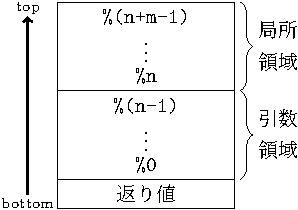
\includegraphics{activeRecord-crop.pdf}
  \end{minipage}
  & \quad &
  \begin{minipage}{.45\textwidth}
    $\texttt{f}(x_1,\cdots,x_n)$でスタック上に
    作成される駆動レコード（の一部）\\
    局所変数: $y_1,\cdots,y_m$\\[10pt]
    \greentext{これに従った記号表を生成}
  \end{minipage}
　\end{tabular}

\vspace*{10pt}

 \begin{description}
   \item [値呼び：]
   $\texttt{x=f(}e_1,\cdots,e_n\texttt{)}$\\
 $e_i$を評価してその値を$x_i$の領域にコピー
   \item [参照呼び：]
   $\texttt{x=f(}z_1,\cdots,z_n\texttt{)}$\\
   $z_i$のアドレスを$x_i$にコピー
 \end{description}
\end{frame}

\begin{frame}[fragile=singleslide]
 \frametitle{引数受渡し}
 \greentext{引数=パラメータ(parameter)}\\
 2種類の受渡し方法
 \begin{list}{}{}
  \item 値渡し：実引数の値を評価して仮引数に代入
  \item 参照渡し：実引数の値を評価して\underline{ポインタ}を仮引数に代入
 \end{list}

\vfill

\begin{center}
\begin{tabular}{ccc}
\multicolumn{1}{c}{値呼び} & \multicolumn{1}{c}{} & \multicolumn{1}{c}{参照呼び}\\\cline{1-1}\cline{3-3}
\multicolumn{1}{|m{.35\textwidth}|}{
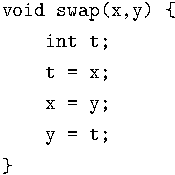
\includegraphics[scale=.8]{swap-value-crop.pdf}
}
& &
\multicolumn{1}{|m{.4\textwidth}|}{
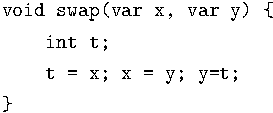
\includegraphics[scale=.8]{swap-ref-crop.pdf}}
\\\cline{1-1}\cline{3-3}
\end{tabular}
\end{center}

\begin{list}{}{}
\item 値呼びの場合：全く効果なし。\\
\greentext{入れ替えられた値は駆動レコード内で実行後破棄}
\item 参照呼びの場合：値が入れ替えられる。\\
\greentext{{\tt swap}中の{\tt y=x}, {\tt x=t}の代入先は、
      実引数の領域}
\end{list}
\end{frame} 

\begin{frame}
  \frametitle{値呼びのコンパイル}
  \%0: xの値，\%1: yの値が格納されているアドレス

\vspace*{5pt}

\begin{center}
  \begin{tabular}{cc}
    \multicolumn{1}{m{.3\textwidth}}{
  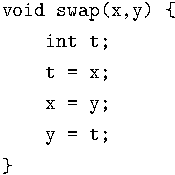
\includegraphics[scale=.8]{swap-value-crop.pdf}}
&
    \multicolumn{1}{m{.5\textwidth}}{
  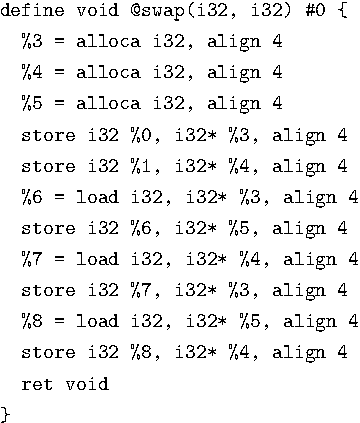
\includegraphics[scale=.7]{swap-v-ll-crop.pdf}}
  \end{tabular}
\end{center}
\end{frame}

\begin{frame}
  \frametitle{参照呼びのコンパイル}
  \%0: xの値，\%1: yの値が格納されているアドレス

\vspace*{5pt}

\begin{center}
  \begin{tabular}{cc}
    \multicolumn{1}{m{.4\textwidth}}{
  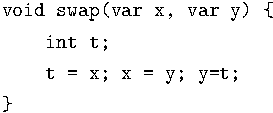
\includegraphics[scale=.8]{swap-ref-crop.pdf}}
&
    \multicolumn{1}{m{.5\textwidth}}{
  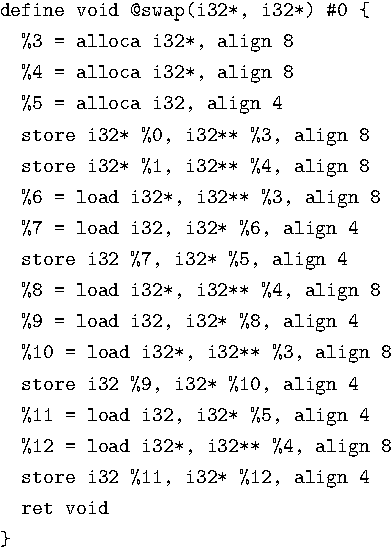
\includegraphics[scale=.7]{swap-ref-ll-crop.pdf}}
  \end{tabular}
\end{center}
\end{frame}

\subsection{関数定義}

\begin{frame}[fragile]{関数定義/値呼び}

  \scalebox{0.75}{
  \begin{tikzpicture}
    \draw[draw] (-0.5,0.5) rectangle (5,-1.5);
    \node[anchor=west] (L01) at (0,0) {\texttt{int add(int x,int y) \{}};
    \node[anchor=west] at (1,-0.5) {\texttt{return x+y;}};
    \node[anchor=west] at (0,-1) {\texttt{\}}};

    \draw[draw] (5.5,0.5) rectangle (13,-5);
    \node[anchor=west] at (6,0) {\texttt{define i32 @add(i32,i32) \{}};
    \node[anchor=west] at (6,-0.5) {\texttt{entry:}};
    \node[anchor=west] at (6.5,-1) {\texttt{\% x = alloca i32}};
    \node[anchor=west] at (6.5,-1.5) {\texttt{\% y = alloca i32}};
    \node[anchor=west] at (6.5,-2) {\texttt{store i32 \% 0, i32* \% x}};
    \node[anchor=west] at (6.5,-2.5) {\texttt{store i32 \% 1, i32* \% y}};
    \node[anchor=west] at (6.5,-3) {\texttt{\% 2 = load i32, i32* \% x}};
    \node[anchor=west] at (6.5,-3.5) {\texttt{\% 3 = load i32, i32* \% y}};
    \node[anchor=west] at (6.5,-4) {\texttt{\% 4 = add i32 \% 2, \% 3}};
    \node[anchor=west] at (6.5,-4.5) {\texttt{ret i32 \% 4}};
  \end{tikzpicture}}
  \parbox{.8\textwidth}{
{\small
関数定義：\\\texttt{define }$\langle$型$\rangle$\texttt{\@}$\langle$関数名$\rangle$(引数型,$\cdots$,引数型)$\rangle$}\\[10pt]
{\small $i$番目の引数 $\% (i-1)$で参照 }
}\\[5pt]
{\small
関数呼出（値呼び）：
\verb|%ret = call i32 @add(%2,%3), align 4|
}
\end{frame}

% \begin{frame}[fragile]
% 	\frametitle{関数定義/値呼出}
% 	\begin{tabular}{c}
% \includegraphics[scale=0.8]{add-c.eps}
% \\[10pt]
% \includegraphics[scale=0.8]{add-function.eps}
% \end{tabular}
% \parbox{.55\textwidth}{
% {\scriptsize
% 関数定義：\\\texttt{define }$\langle$型$\rangle$\texttt{\@}$\langle$関数名$\rangle$(引数型,$\cdots$,引数型)$\rangle$}\\[10pt]
% $i$番目の引数 $\% (i-1)$で参照
% }\\[5pt]
% 関数呼出（値呼び）：
% \verb|%ret = call i32 @add(%2,%3), align 4|
% \end{frame}

% \begin{frame}{関数定義/参照呼出}
%   \scalebox{0.7}{
%     \begin{tikzpicture}
%       \draw[draw] (-0.5,0.5) rectangle (5.5,-2.5);
%       \node[anchor=west] (L01) at (0,0) {\texttt{int add(int *x,int *y) \{}};
%       \node[anchor=west] at (1,-0.5) {\texttt{int t;}};
%       \node[anchor=west] at (1,-1) {\texttt{t = *x;}};
%       \node[anchor=west] at (1,-1.5) {\texttt{*x = *y;}};
%       \node[anchor=west] at (1,-2) {\texttt{*y = t;}};
  
%       \draw[draw] (6,0.5) rectangle (15,-9);
%       \node[anchor=west] at (6.5,0) {\texttt{define vod @swap(i32*,i32*) \{}};
%       \node[anchor=west] at (7,-0.5) {\texttt{\% 3 = alloca i32*, align 8}};
%       \node[anchor=west] at (7,-1) {\texttt{\% 4 = alloca i32*, align 8}};
%       \node[anchor=west] at (7,-1.5) {\texttt{\% 5 = alloca i32, align 4}};
%       \node[anchor=west] at (7,-2) {\texttt{store i32* \% 0, i32** \% 3, align 8}};
%       \node[anchor=west] at (7,-2.5) {\texttt{store i32* \% 1, i32** \% 4, align 8}};
%       \node[anchor=west] at (7,-3) {\texttt{\% 6 = load i32*, i32** \% 3, align 8}};
%       \node[anchor=west] at (7,-3.5) {\texttt{\% 7 = load i32, i32* \% 6, align 4}};
%       \node[anchor=west] at (7,-4) {\texttt{store i32 \% 7, i32* \% 5, align 4}};
%       \node[anchor=west] at (7,-4.5) {\texttt{\% 8 = load i32*, i32** \% 4, align 8}};
%       \node[anchor=west] at (7,-5) {\texttt{\% 9 = load i32, i32* \% 8, align 4}};
%       \node[anchor=west] at (7,-5.5) {\texttt{\% 10 = load i32*, i32** \% 3, align 8}};
%       \node[anchor=west] at (7,-6) {\texttt{store i32 \% 9, i32* \% 10, align 4}};
%       \node[anchor=west] at (7,-6.5) {\texttt{\% 11 = load i32, i32* \% 5, align 4}};
%       \node[anchor=west] at (7,-7) {\texttt{\% 12 = load i32*, i32** \% 4, align 8}};
%       \node[anchor=west] at (7,-7.5) {\texttt{store i32 \% 11, i32* \% 12, align 4}};
%       \node[anchor=west] at (7,-8) {\texttt{ret void}};
%       \node[anchor=west] at (6.5,-8.5) {\texttt{\}}};
%     \end{tikzpicture}}
% \end{frame}

% \begin{frame}[fragile]
% 	\frametitle{関数定義/参照呼出}
% 	\begin{tabularx}{\textwidth}{|X|c|X|}\cline{1-1}\cline{3-3}
% 	\includegraphics[width=.4\textwidth]{swap-ref-ll.eps}& &
% 	\includegraphics[width=.4\textwidth]{swap-ref.eps}\\\cline{1-1}\cline{3-3}
% 	\end{tabularx}
% \end{frame}

% \section{型}

% \subsection{型定義}

% \begin{frame}[fragile]
%  \frametitle{型(Type)}


%  プログラミング言語における型に関する情報
%  \begin{list}{}{}
%   \item [型検査:] プログラムの識別子(変数、関数名など)の一貫
% 	性
% 	\begin{verbatim}
% int x; char c; float y;
% x = y + c;
% 	\end{verbatim}
%   \item [変換への適用:] 変数が必要とするメモリ領域量
% 	\begin{tabular}{rl}
% 	\verb|int|: & 32ビットまたは64ビット\\
% 	\verb|char|: & 8ビットまたは16ビット\\
% 	\verb|float|: & 32ビット(符号1,指数8,仮数23)\\
%         \verb|double|: & 64ビット (符号1,指数11,仮数52)
% 	\end{tabular}
% 	% \begin{pspicture}(0,0)(8,1)
% 	%  \psframe(0,0)(8,0.5)
% 	%  \psline(0.5,0)(0.5,0.5)
% 	%  \psline(1,0)(1,0.5)
% 	%  \rput(1.75,0.25){$\cdots$}
% 	%  \psline(2.5,0)(2.5,0.5)
% 	%  \psline(3,0)(3,0.5)
% 	%  \psline(3.5,0)(3.5,0.5)
% 	%  \rput(5.5,0.25){$\cdots$}
% 	%  \psline(7.5,0)(7.5,0.5)
% 	%  \psline(0,0.5)(0.1,0.6)(0.4,0.6)(0.5,0.5)
% 	%  \rput(0.25,0.8){\scriptsize 符号}
% 	%  \psline(0.5,0.5)(0.6,0.6)(2.9,0.6)(3,0.5)
% 	%  \rput(1.75,0.8){\scriptsize 指数}
% 	%  \psline(3,0.5)(3.1,0.6)(7.9,0.6)(8,0.5)
% 	%  \rput(5.5,0.8){\scriptsize 仮数}
% 	% \end{pspicture}
%  \end{list}
% \end{frame}

% \begin{frame}[fragile]
% \frametitle{型の意味}

% \begin{enumerate}
%  \item 型から領域の大きさを知ることができる。
%  \item 構造体,レコードなどのデータ構造
%  \item 配列宣言によるデータ領域
% \end{enumerate}

% 	\verb|x = y + c | という式は妥当か？\\
% 	\greentext{構文木は構成可能であるが、意味的に誤り\\
% '加算'の意味が定義できない}

% \greentext{再帰的データ構造}:木構造、リスト構造

% \vspace*{1zw}

% \begin{tabular}{cc}
% \begin{minipage}{.6\textwidth}
% \begin{verbatim}
% struct NODE {
%    DATATYPE data;
%    struct NODE *leftchild;
%    struct NODE *rightchild;
% }
% \end{verbatim}
% \end{minipage}
%  &
%  \begin{minipage}{.4\textwidth}
% \begin{verbatim}
% struct NODE {
%    DATATYPE data;
%    struct NODE *next;
% }
% \end{verbatim}
% \end{minipage}
% \end{tabular}
% \end{frame}

% \begin{frame}[fragile]
%  \frametitle{型宣言}

% 配列とポインタを含む型宣言を考える．

%  \begin{eqnarray*}
%   D & \rightarrow & T\ \mathsf{id}\ ;\ D\ |\ \varepsilon\\
%   T & \rightarrow & \mathtt{int}\ |\ \mathtt{char}\ |\ TC\ |\ \mathtt{\&}T\\
%   C & \rightarrow & \varepsilon\ |\ \mathtt{[}\ \mathsf{num}\ \mathtt{]}C\\
%  \end{eqnarray*}

% 型宣言：\texttt{int x; int[10] y; \&char[3][10] z;}

%  それぞれの型式：\\
%  x:\greentext{\sf integer}\\
%  y:\greentext{\sf array(0..9,integer)}\\ 
%  z:\greentext{\sf
%  array(0..2,array(0..9,$\uparrow$character))}\\

%  \vspace*{1zw}

%  C言語：\texttt{int x;int y[10];char *z[3][10];}
% \end{frame}

% \begin{frame}[fragile]
%  \frametitle{型属性の計算}
%  型宣言の意味規則として計算する．（64ビットマシンを想定)
%  \[
%   \begin{array}{rclp{.7\textwidth}}
%    T & \rightarrow & T_1 & $\{t=T_1.type;w=T_1.size\}$\\
%      &             & C & $\{T.type=C.type;T.width=C.size\}$\\
%    T & \rightarrow & \mathtt{\&}T_1 &
%     $\{T.type=\mathsf{pointer}(T_1.type);\newline T.size=8\}$\\
%    B & \rightarrow & \mathtt{int} &
%     $\{B.type=\mathsf{integer};B.size=8\}$\\
%    B & \rightarrow & \mathtt{char} &
%     $\{B.type=\mathsf{real};B.size=1\}$\\
%    C & \rightarrow & \varepsilon &
%     $\{C.type=t;C.size=w\}$\\
%    C & \rightarrow & [\mathsf{num}]C_1 &
%     $\{C.type=\mathsf{array(0..num}.value-1,C_1.type\mathsf{)};\newline
%     C.size=\mathsf{num}.value\times C_1.size\}$\\
%   \end{array}
%  \]
%  \verb|&int[10][30]|.type={\sf array}(0..9,{\sf
%  array}(0..29,{\sf integer})),\\
%  \verb|&int[10][30]|.size=2400

%  \vspace*{3mm}

%  \greentext{記号表にこのような属性を登録する}
% \end{frame}

% \begin{frame}
% \frametitle{式の型}

% \[
%  \begin{array}{rcl}
%   P & \rightarrow & D;E\\
%  D & \rightarrow & T\ \mathsf{id}\ ;\ D\ |\ \varepsilon\\
%  T & \rightarrow & \mathtt{int}\ |\ \mathtt{char}\ |\ TC\ |\ \mathtt{\&}T\\
%  C & \rightarrow & \varepsilon\ |\ \mathtt{[}\ \mathsf{num}\ \mathtt{]}C\\
%   E & \rightarrow & \mathsf{c}\ |\ \mathsf{n}\ |\ \mathsf{id}\ |\ E+E\
%    |\ \mathtt{\&}E\ |\ \mathtt{\ast}E\ |\ E[E]\\
%  \end{array}
% \]

% \[
%  \begin{array}{rc}
%   \mathtt{int}\ i;i+(1+2) & \only<2->{\mbox{OK}}\\
%   \mathtt{\& int}\ i;i+4 & \only<3->{\mbox{NG}}\\
%   \mathtt{int[10]}\ a;\mathtt{int}\ k;a[k]+3 & \only<4->{\mbox{OK}}\\
%   \mathtt{\& int[10]}\ a;\mathtt{\&\& int[4]}\ b;\ast\ast a[\ast b] &
%    \only<5->{\mbox{NG}}\\
%  \end{array}
% \]

% \end{frame}

% \begin{frame}
% \frametitle{意味規則による型検査}
% \[
% \begin{array}{lp{.8\textwidth}}
%  E\rightarrow\mathsf{c} & $E.type=\mathtt{char}$\\
%  E\rightarrow\mathsf{n} & $E.type=\mathtt{int}$\\
%  E\rightarrow\mathsf{id} & $E.type=\mathsf{id}.type$\\
%  E\rightarrow E_1+E_2 & $E.type=\mathbf{if}\ E_1.type=\mathtt{int}\
%   \mathrm{and}\ E_2.type=\mathtt{int}\newline
%   \mathbf{then}\ \mathtt{int}\ \mathbf{else}\ \mathtt{error}$\\
%  E\rightarrow \mathtt{\&}E_1 & $E.type=\mathsf{pointer}(E_1.type)$\\
%  E\rightarrow \mathtt{\ast}E_1 & $\mathbf{if}\ t\ exists\ such\ that
%   \mathsf{pointer}(t)=E_1.type\newline
%   \mathbf{then}\ E.type=t\ \mathbf{else}\ \mathtt{error}$\\
%  E\rightarrow E_1[E_2] &
%   $E.type=\mathbf{if}\ E_1.type=\mathsf{array}(s,t)\ \mathrm{and}\
%   E_2.type=\mathtt{int}\ \mathbf{then}\ t\ \mathbf{else}\ \mathtt{error}$
% \end{array}
% \]
% \end{frame}

% \begin{frame}[fragile]
% \frametitle{柔軟な型の扱い}
% 型を厳密に扱うこと：\\
% コンパイラとしては有利だが、プログラマには負担l\\
% \greentext{型に対するポリシー=プログラミング言語設計の基本概
% 念の1つ}
% \begin{list}{$\cdot$}{}
%  \item{型変換}
%       意味として互換性を持つデータ型についてエラーとせず、型を変換
%       して適当な意味を割り当てる。
%       \begin{list}{}{}
% 	\item 派生型(subtype)：$S<:T$\\
% 	      $\mathtt{int}<:\mathtt{float}$
% %	\item オブジェクト指向言語におけるサブクラス (is-a関
% %	      係)
% 	      $\mathtt{func}(T\ x):S$に対して、$T'<:T$となる型$T'$の
% 	      適用を許す。$S<:S'$となる型$S'$の返り値を許す。\\
%       \end{list}
%       \verb|float x,z;int y;z=x+y;y=x-z;|(1番目OK, 2番目NG)
%  \item{多相型(Polymorphic type)}:
%       いろいろな型を受け取る関数\\
%       \verb|function len(x)=if null(x) then 0 else len(tl(x))+1|\\
%       ${\tt tl}$:tail関数 先頭の要素だけを除いたものを返す\\
%       \greentext{\small tail関数が適用できる型ならば{\tt len}を適用可
%       能}
% \end{list}
% \end{frame}

% \subsection{配列の型}

% \begin{frame}[fragile]
%  \frametitle{配列型データの参照}
%  1次元配列 $\mathtt{a}[n]$=$\mathtt{a}.addr+n-1$\\
%  2次元配列
%  $\mathtt{b}[m][n]$=$\mathtt{b}.addr+\mathtt{C1}\times
%  m+n-1$(横優先)\\
% % ここで、$\mathtt{int[C1][C2]}\ b$と宣言されているとする。\\
%  $\mathtt{b}[m][n]$=$\mathtt{b}.addr+\mathtt{C2}\times
%  n+m-1$(縦優先)

% %\begin{center}
% % \includegraphics[scale=0.8]{figs191113/array-fig.eps}
% %\end{center}

% \begin{center}
% \scalebox{0.5}{
% \begin{tikzpicture}
% \node at (1,4) {b[0][0]};
% \node at (1,3) {b[1][0]};
% \node at (1,2) {$\vdots$};
% \node at (1,1) {b[98][0]};
% \node at (1,0) {b[99][0]};
% \node at (3,4) {b[0][1]};
% \node at (3,3) {b[1][1]};
% \node at (3,2) {$\vdots$};
% \node at (3,1) {b[98][1]};
% \node at (3,0) {b[99][1]};
% \node at (5,4) {$\cdots$};
% \node at (5,3) {$\cdots$};
% \node at (5,2) {$\ddots$};
% \node at (5,1) {$\cdots$};
% \node at (5,0) {$\cdots$};
% \node at (7,4) {b[0][98]};
% \node at (7,3) {b[1][98]};
% \node at (7,2) {$\vdots$};
% \node at (7,1) {b[98][98]};
% \node at (7,0) {b[99][98]};
% \node at (9,4) {b[0][99]};
% \node at (9,3) {b[1][99]};
% \node at (9,2) {$\vdots$};
% \node at (9,1) {b[98][99]};
% \node at (9,0) {b[99][99]};
% \path[->] (-0.5,4.5) edge [below,sloped] node {縦優先} (-0.5,-0.5);
% \path[->] (0,4.5) edge [above] node {横優先} (9.5,4.5);
% \node[anchor=east] at (-0.7,4.5) {C1=C2=100};
% \end{tikzpicture}
% }
% \end{center}
 
% % \[
% % \begin{array}{cccccc}
% %  b[0][0] & b[0][1] & \cdots & b[0][\mathtt{C2}-2] & b[0][\mathtt{C2}-1]\\
% %  b[1][0] & b[1][1] &        & b[1][\mathtt{C2}-2] & b[1][\mathtt{C2}-1]\\
% %   \vdots & \vdots  &        &    \vdots           &  \vdots\\
% %  b[\mathtt{C1}-2][0] & b[\mathtt{C1}-2][1] &  & b[\mathtt{C1}-2][\mathtt{C2}-2] & b[\mathtt{C1}-2][\mathtt{C2}-1]\\
% %  b[\mathtt{C1}-1][0] & b[\mathtt{C1}-1][1] &  & b[\mathtt{C1}-1][\mathtt{C2}-2] & b[\mathtt{C1}-1][\mathtt{C2}-1]\\
% % \end{array}
% % \]
% % 多次元配列は、メモリ上に1列にならべる。
% %
% % どの次元から並べるかは任意性がある。

%  \greentext{ループで回すときには、実行性能に差が出ることがあ
%  る。}

% %  {\small
% % \texttt{for(int i=0;i<C1,i++) for(int j=0;j<C2,j++)} b[i][j]へのアクセス
% %  }

% {\tt C1}、{\tt C2}が大きい場合：\\
% \greentext{横優先のとき内側のループはキャッシュ内におさまる
%  可能性大}\\
% \greentext{縦優先のとき主記憶へのアクセスが発生する可能性大}

% \end{frame}

% \begin{frame}
%  \frametitle{インデックス修飾}

%  \texttt{a[n] = a.addr + n - 1}
 
%  \vspace*{10pt}
 
%  \texttt{a.addr}:ベースアドレス
 
%  \texttt{n-1}：インデックス
 
%  \vspace*{10pt}
 
%  使用頻度が高いのでハードウェアで実現されることも多い
%  (初期のマイクロコンピュータなど）
 
%  \vspace*{10pt}

%  アドレス計算；ベースレジスタ+相対番地+インデックスレジスタ

%  \greentext{配列の位置計算を高速に行いたい}

% \vspace*{10pt}

% LLVM: \texttt{getelementptr}を用いる．

% \end{frame}

\section{コード最適化}

\begin{frame}
  \begin{center}
  {\Huge コード最適化}
  \end{center}
\end{frame}

\subsection{概要}

\begin{frame}
 \frametitle{コード最適化}
 
 実行の意味を変えることなく実行を高速化すること。

 \begin{list}{}{}
  \item 実行の意味：入力と出力\\
	最適化の対象によって入力と出力は変わる。\\
	\greentext{プログラム解析が必要}
 \end{list}


 \begin{itemize}
  \item 機械独立なコード最適化\\
	\quad =3番地コードのレベルで実行を効率化
  \item 機械依存なコード最適化\\
	\quad =対象マシンのアーキテクチャに依存\\
	\qquad (VLIW、マルチコアなど)
 \end{itemize}

\end{frame}

\subsection{局所最適化}

\begin{frame}
 \frametitle{基本ブロック}

 最後以外分岐のない文の並び

\begin{center}
 \only<1>{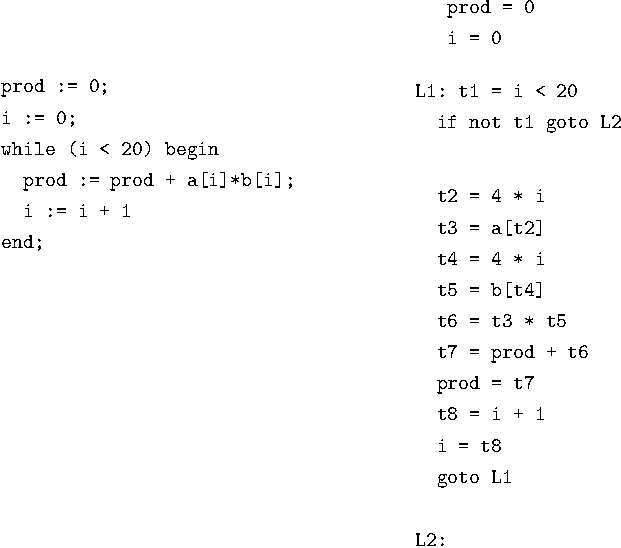
\includegraphics[width=.8\textwidth]{basic-block-fig-r2-crop.pdf}}
 \only<2>{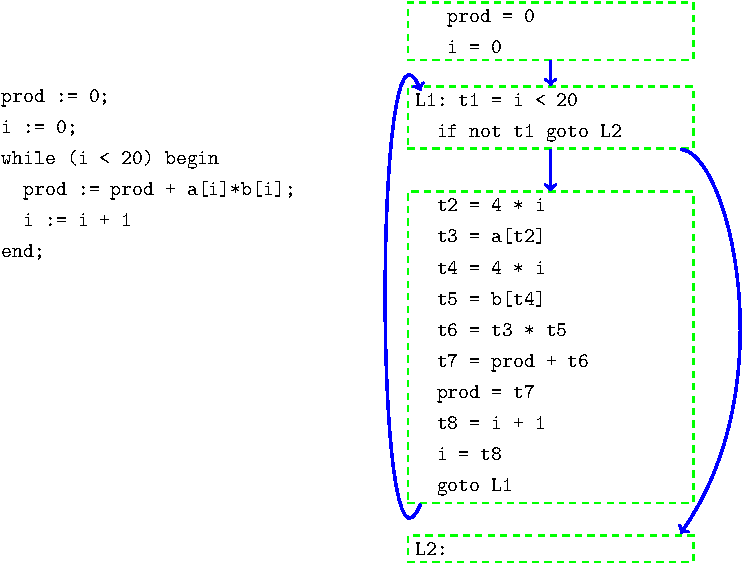
\includegraphics[width=.8\textwidth]{basic-block-fig2-r2-crop.pdf}}
\end{center}

\end{frame}

\begin{frame}
 \frametitle{局所最適化}

 基本ブロック内だけを見て最適化すること

 覗き穴最適化(Peep-hole optimization)

 \begin{itemize}
  \item 定数伝播(constant propagation)\\
	\greentext{定数の計算、参照を定数そのものでおきかえる}
  \item 共通部分式の削除(common subexpression elimination)\\
	\greentext{共通の部分式を抽出して結果を一時変数に保存
	するようにして、二回目以降計算しない。}
  \item コピー伝播(copy propagation)\\
	\greentext{余分な変数の仲介を減らす。}\\
	\greentext{データ依存性を減らして命令の並列発行が可能
	になる場合がある。}
  \item 不要コードの除去(deadcode elimination)\\
	\greentext{使われない変数に関する計算を消去する。}
  \item 代数的性質の利用\\
	\greentext{演算子が持つ代数的性質(可換則、結合則、分
	配則、計算のためのコストなど)}
 \end{itemize}
\end{frame}

\begin{frame}
 \frametitle{DAGによる局所最適化}

 DAG=Directed Asyclic Graph\\
 \greentext{閉路(ループ)をもたない有効グラフ}

 \greentext{基本ブロック内のデータ依存性を一意的に表現}

 DAGの構成アルゴリズム 6.6


\end{frame}

\begin{frame}
 \frametitle{DAGの構成}
 \begin{tabular}{cc}
 \begin{minipage}{.45\textwidth}

  \begin{tikzpicture}
   \node[draw,circle] (a0) at (0,0) {$a_0$};
   \node[draw,circle] (b0) at (1.5,0) {$b_0$};
   \node[draw,circle] (c0) at (3,1) {$c_0$};
   \uncover<2->{\node[draw,circle] (AST) at (0.75,1) {$\ast$};}
   \uncover<2-6>{\node at ($(AST)+(0.5,0)$) {$x$};}
   \uncover<3->{\node[draw,circle] (PLUS) at (2,2) {$+$};
     \node at ($(PLUS)+(0.5,0)$) {$y$};}
   \uncover<4->{\node at ($(AST)+(0.8,0)$) {$,d$};}
   \uncover<5->{\node[draw,circle] (MIN) at (2,3.5) {$-$};
     \node at ($(MIN)+(0.5,0)$) {$e$};}
   \uncover<7->{\node[draw,circle] (PL2) at (2,5) {$+$};
   \node at ($(PL2)+(0.5,0)$) {$x$};}
   \only<2->{
   \path[-] (a0) edge (AST) (b0) edge (AST);
   }
   \only<3->{
   \path[-] (AST) edge (PLUS) (c0) edge (PLUS);
   }
   \only<5->{
   \path[-] (MIN) edge (AST) (MIN) edge (c0);
   }
   \only<7->{
   \path[-] (PL2) edge (AST) (PL2) edge (MIN);
   }
  \end{tikzpicture}

 \end{minipage}
  &
   \begin{minipage}{.4\textwidth}

    \begin{tikzpicture}
     \node[anchor=west] at (0,3) {\texttt{x=\redtext{a}*\redtext{b}}};
     \only<1,3->{\node[anchor=west] at (0,2.5) {\texttt{y=x+\redtext{c}}};}
     \only<1,4->{\node[anchor=west] at (0,2) {\texttt{d=\redtext{a}*\redtext{b}}};}
     \only<1,5->{\node[anchor=west] at (0,1.5) {\texttt{e=d-\redtext{c}}};}
     \only<1,7->{\node[anchor=west] at (0,1) {\texttt{x=d+e}};}

     \only<6>{
     \node at (2,2.5) {$\Rightarrow$};
     \node[anchor=west] at (3,3) {\texttt{x=a*b}};
     \node[anchor=west] at (3,2.5) {\texttt{y=x+c}};
     \node[anchor=west] at (3,2) {\texttt{d=x}};
     \node[anchor=west] at (3,1.5) {\texttt{e=d-c}};
     }

     \only<7>{
     \node[anchor=west] at (3,3) {\texttt{d=a*b}};
     \node[anchor=west] at (3,2.5) {\texttt{y=d+c}};
     \node[anchor=west] at (3,2) {\texttt{e=d-c}};
     \node[anchor=west] at (3,1.5) {\texttt{x=d+e}};
     }

    \end{tikzpicture}

   \end{minipage}
 \end{tabular}
\end{frame}

\begin{frame}
 \frametitle{不要コードの消去}
 \begin{tabular}{cc}
  \parbox{.3\textwidth}{これ以降、$x$しか使用しないとすると
  \only<2>{$\mathtt{y=d+c}$は消去}}
  \begin{minipage}{.4\textwidth}

   \begin{tikzpicture}
    \only<1,2>{\node[draw,circle] (a0) at (0,0) {$a_0$};
    \node[draw,circle] (b0) at (1.5,0) {$b_0$};
    \node[draw,circle] (c0) at (3.25,1) {$c_0$};
    \node[draw,circle] (AST) at (0.75,1) {$\ast$};
    \node[draw,circle] (MIN) at (2,3.5) {$-$};
    \node[draw,circle] (PL2) at (2,5) {$+$};
    \node at ($(AST)+(0.5,0)$) {$d$};
    \node at ($(MIN)+(0.5,0)$) {$e$};
    \node at ($(PL2)+(0.5,0)$) {$x$};
    \path[-] (a0) edge (AST) (b0) edge (AST)
             (AST) edge (MIN) (c0) edge (MIN)
             (AST) edge (PL2) (MIN) edge (PL2);
    }
    \only<1>{\node[draw,circle] (PL1) at (2,2) {$+$};
    \node at ($(PL1)+(0.5,0)$) {$y$};
    \path[-] (AST) edge (PL1)  (c0) edge (PL1);
    }
    
   \end{tikzpicture}

  \end{minipage}
  &
   \begin{minipage}{.4\textwidth}

    \begin{tikzpicture}
     \node[anchor=west] at (0,3.5) {\texttt{d=a*b}};
     \only<1>{\node[anchor=west] at (0,3.1) {\texttt{y=d+c}};}
     \node[anchor=west] at (0,2.7) {\texttt{e=d-c}};
     \node[anchor=west] at (0,2.3) {\texttt{x=d+e}};
    \end{tikzpicture}

   \end{minipage}
 \end{tabular}

 \vspace*{10pt}

 \greentext{不要な変数を上からたどって消していく。}\\
 \greentext{$e$,$d$は直接使わないが、$x$の計算に必要なので消去できない。}
\end{frame}

\begin{frame}
 \frametitle{代数的性質}
 \begin{center}
 \begin{tabular}{ccc}
 \begin{minipage}{.3\textwidth}
  \scalebox{0.8}{
  \begin{tikzpicture}
   \node[draw,circle] (a0) at (0,0) {$a_0$};
   \node[draw,circle] (b0) at (1.5,0) {$b_0$};
   \node[draw,circle] (c0) at (3,0) {$c_0$};
   \node[draw,circle] (AS1) at (0.75,1) {$\ast$};
   \node[draw,circle] (AS2) at (2.25,1) {$\ast$};
   \node[draw,circle] (PL) at (1.5,2) {$+$};
   \path[-] (a0) edge (AS1)  (b0)edge (AS1)  (b0) edge (AS2)
            (c0) edge (AS2)  (AS1) edge (PL) (AS2) edge (PL);
  \end{tikzpicture}
  }
 \end{minipage}
  &
  $\Rightarrow$
 &
 \begin{minipage}{.3\textwidth}
  \scalebox{0.8}{
  \begin{tikzpicture}
   \node[draw,circle] (a0) at (0,0) {$a_0$};
   \node[draw,circle] (c0) at (1.5,0) {$c_0$};
   \node[draw,circle] (b0) at (3,0) {$b_0$};
   \node[draw,circle] (PL) at (0.75,1) {$+$};
   \node[draw,circle] (AS) at (1.5,2) {$\ast$};
   \path[-] (a0)edge (PL)  (c0)edge (PL) (PL) edge  (AS) (b0) edge (AS);
  \end{tikzpicture}
  }
 \end{minipage}\\
  \begin{minipage}{.3\textwidth}
\begin{tabular}{l}
{\tt t1=a*b}\\
{\tt t2=b*c}\\
{\tt t3=t1+t2}\\
\end{tabular}
  \end{minipage}
& &
  \begin{minipage}{.3\textwidth}
\begin{tabular}{l}
{\tt t1=a+c}\\
{\tt t2=t1*b}
\end{tabular}
  \end{minipage}
  \end{tabular}

\vspace*{1zw}

\par\noindent
\greentext{分配則=DAG上でのパターンマッチング}
 \end{center}
 \end{frame}

% \begin{frame}[fragile]
%  \frametitle{配列参照}

% \begin{enumerate}
%  \item $\mathtt{x = a[i]}$の形の配列参照\\
%        演算子\texttt{=[]}のノードを生成し、子として$a_0$および$i$、
%        ノードに$x$をラベルづけする。
%  \item \texttt{a[i]=x}の形の配列代入\\
%        演算子\texttt{[]=]}のノードを生成し、
%        子として、$a_0$, $i$, $x$をとり、$a_0$を参照している
%        \texttt{=[]}ノードに'killed'マークをつける。
%        $a[i]$は共通部分式として用いることはできない。
% \end{enumerate}

%  \vspace*{0.5cm}

%  \begin{tabular}{ccc}
%  \begin{tabular}{l}
% {\tt x = a[i]}\\
% {\tt a[j]=y}\\
% {\tt z=a[i]}
%  \end{tabular}
%   & \hspace*{1cm} &

% \begin{tikzpicture}
%  \node (a0) at (0,0) {$a_0$};
%  \node (i0) at (1.5,0) {$i_0$};
%  \node (j0) at (3,0) {$j_0$};
%  \node (y0) at (4.5,0) {$y_0$};

%  \node[draw] (Ar1) at (0.75,1) {\texttt{=[]}};
%  \node[draw] (Ar2) at (3.75,1) {\texttt{=[]}};

%  \node[draw] (Ar3) at (0.75,2.5) {\texttt{=[]}};
 
%  \node (Ann0) at (0.75,1.5) {\sf Killed};

%  \node at ($(Ar1)+(0.8,0)$) {$x$};
%  \node at ($(Ar3)+(0.8,0)$) {$z$};

%  \path (a0) edge (Ar2)  (i0) edge (Ar2)  (j0) edge (Ar2) (y0) edge (Ar2);
%  \path (a0) edge (Ar1)  (i0) edge (Ar1);
%  \path (a0) [out=120,in=225] edge (Ar3);
%  \path (i0) [out=60, in=315] edge (Ar3);
% \end{tikzpicture}
%  \end{tabular}
 
% \end{frame}

% \subsection{大域的最適化}
 
%  \begin{frame}
%  \frametitle{大域的コード最適化}
%  基本ブロックを越える最適化

%  \begin{list}{}{}
%   \item ループ最適化
%   \item 手続き呼び出し最適化
%   \item データフロー解析
%   \item 静的単一代入(SSA)解析
%  \end{list}
% \end{frame}

% \begin{frame}
%  \frametitle{ループ最適化(1/3)}
%  ループ内のコード実行回数:ループ外のコードよりも一般に多い\\
%  ループ内のコードは慎重に最適化\\
%  本当に毎回実行しなければならないか？できるだけ効率よく実行
%  \begin{list}{}{}
%   \item ループ不変式の移動\\
% 	\greentext{ループから影響をうけない式を外に出す}l\\
% 	例6.8
%   \item ループ内の演算の強さの軽減\\
% 	強い演算：時間のコストが大きい演算\\
% 	足し算$<$掛け算 (加算器$<$乗算器)\\
% 	例6.9
%  \end{list}
% \end{frame}

% \begin{frame}
%  \frametitle{例}
%  \begin{center}
%  \begin{tabular}{ccc}
%   \multicolumn{3}{l}{例6.8}\\
%   \includegraphics[scale=.7]{ex6_8_1.eps}
%   & $\Rightarrow$ & 
%   \includegraphics[scale=.7]{ex6_8_2.eps} \\[1zw]
%   \includegraphics[scale=.7]{ex6_8_3.eps}
%   & $\Rightarrow$ & 
%   \includegraphics[scale=.7]{ex6_8_4.eps} \\[1zw]
%   \multicolumn{3}{l}{例6.9}\\
%   \includegraphics[scale=.7]{ex6_9_1.eps}
%   & $\Rightarrow$ & 
%   \includegraphics[scale=.7]{ex6_9_2.eps}
%  \end{tabular}
%  \end{center}
% \end{frame}

% \begin{frame}
%  \frametitle{ループ最適化(2/3)}
%  \begin{list}{}{}
%   \item 帰納変数消去\\
% 	\greentext{帰納変数(ループを制御する変数)は減らす。}\\
% 	\greentext{参照数の減少}
% 	\begin{center}
% 	 \begin{tabular}{ccc}
% 	  \includegraphics[scale=.75]{ex6_10_1.eps}
% 	  & $\Rightarrow$ &
% 	  \includegraphics[scale=.75]{ex6_10_2.eps}
% 	 \end{tabular}
% 	\end{center}
	
%   \item ループ融合とループ分離\\
%   \item ループ展開とソフトウェアパイプライン
%  \end{list}
% \end{frame}

% \begin{frame}
%  \frametitle{ループ展開とソフトウェアパイプライン}
%  \begin{center}
%  \begin{tabular}{ccc}
%   \includegraphics[scale=.75]{ex6_14_1.eps}
%   & $\Rightarrow$ &
%   \includegraphics[scale=.75]{ex6_14_2.eps}
%  \\
%  \end{tabular}

%   \[
%    \begin{array}{c|ccc}
%     &P_1 &P_2 &P_3 \\\hline
%    1 & A_1 & & \\
%    2 & B_1 & A_2 & \\
%    3 & C_1 & B_2 & A_3 \\
%    4 & A_4 & C_2 & B_3 \\
%    5 & B_4 & A_5 & C_3 \\
%    \vdots & \multicolumn{3}{c}{\vdots}\\
%    \end{array}
%   \]
%  並列に実行可能
%  \end{center}
% \end{frame}

% \begin{frame}
%  \frametitle{手続き呼出し最適化}

%  \begin{list}{}{}
%   \item {\bf インライン展開}:\ \\
%  手続き呼出し=駆動レコードを用いてスタック上に情報を保存

%  \greentext{操作としてはコストが大きい}

%  スタック操作：実メモリへの正確な順序での書き込みを要求

%  短い手続きや関数であればそのまま置き換えてしまった方が
%  効率がよい。

%   \item {\bf 末尾再帰}:\\

% 	手続の最後の再帰よびだしは、gotoに置き換え可能。
	
% 	\greentext{呼出しから復帰しても駆動レコード上の局所環境を使って
% 	実行する命令が存在しない。局所領域も再利用可能}
%  \end{list}

% \end{frame}

% \begin{frame}
%  \frametitle{末尾再帰の例}
%  \begin{tabular}{ccc}
%   \includegraphics[scale=.6]{ex6_16_1.eps}
%   & $\Rightarrow$ &
%   \includegraphics[scale=.6]{ex6_16_2.eps}\\
%   & & $\Downarrow$\\
%   & &
%   \includegraphics[scale=.6]{ex6_16_3.eps}
%  \end{tabular}
% \end{frame}

% \subsection{データフロー解析}

% \begin{frame}
%  \frametitle{データフロー解析}

%  \vspace*{10pt}

%  \greentext{(教科書6.4:詳細については省略)}

%  \vspace*{10pt}

%  ステートメント$S$に対するデータフロー

%  \[
%   out[S]=gen[S]\cup(in[S]-kill[S])
%  \]

%  プログラム上での位置(行番号)：
%  \begin{tabular}{ll}
%   $in[S]$ & $S$に入力されるデータ\\
%   $out[S]$ & $S$から出力されるデータ\\
%   $gen[S]$ & $S$で定義されるデータ\\
%   $kill[S]$ & $S$で上書きされるデータ\\
%  \end{tabular}

%  入力から出力への制御がきまっていればよいので、基本ブロック単位で考えれ
%  ばよい。

%  ループ：データフロー方程式を解いて全体的に必要なデータを計算する。
% \end{frame}

% \begin{frame}{データフロー方程式}
% % \begin{tabular}{ccc}
% %  \begin{minipage}{.2\textwidth}
% % \begin{tikzpicture}
% %  \node[draw] (S1) at (0,1.5) {$S_1$};
% %  \node[draw] (S2) at (0,0) {$S_2$};
% %  \path[->] (S1) edge (S2);
% % \end{tikzpicture}
% %  \end{minipage}
% %  &
% %  \begin{minipage}{.25\textwidth}
% %   \begin{tikzpicture}
% %    
% %   \end{tikzpicture}
% %  \end{minipage}
% % \end{tabular}

% \scalebox{0.7}{
% \begin{tikzpicture}
%  \node[draw] (B5) at (2,0) {EXIT};
%  \node[draw] (B4) at (2,1) {$d_7$:\texttt{i=u3}};
%  \node[draw] (B3) at (0,2) {$d_6$:\texttt{a=u2}};
%  \node[draw] (B2) at (2,3.25) {$\begin{array}{ll}
%   d_4: & \texttt{i=i+1}\\[-3pt]
%   d_5: & \texttt{j=j-1}
% 		       \end{array}$};
%  \node[draw] (B1) at (2,5) {$\begin{array}{ll}
%   d_1: & \texttt{i=m-1}\\[-3pt]
%   d_2: & \texttt{j=n}\\[-3pt]
%   d_3: & \texttt{a=u1}
% 			\end{array}$};
%  \node[draw] (B0) at (2,6.5) {ENTRY};

%  \node at ($(B1)+(1.5,0)$) {$B_1$};
%  \node at ($(B2)+(1.5,0)$) {$B_2$};
%  \node at ($(B3)+(1.2,0)$) {$B_3$};
%  \node at ($(B4)+(1.2,0)$) {$B_4$};

%  \path[->] (B0) edge (B1) (B1) edge (B2) (B2) edge (B4)
%            (B2) edge (B3) (B3) edge (B4) (B4) edge (B5);
%  \path[->] (B4) [out=210,in=150,looseness=3] edge (B2);

%  \node[anchor=west] at ($(B1)+(2.5,0)$) {$\begin{array}{ll}
%   gen_{B_1} & = \{d_1,d_2,d_3\}\\[-3pt]
%   kill_{B_1} & = \{d_4,d_5,d_6,d_7\}
% 			   \end{array}$};
%  \node[anchor=west] at ($(B2)+(2.5,0)$) {$\begin{array}{ll}
%   gen_{B_2} & = \{d_4,d_5\} \\[-3pt]
%   kill_{B_2} & = \{d_1,d_2,d_7\}
% 			   \end{array}$};
%  \node[anchor=west] at ($(B3)+(4.5,0)$) {$\begin{array}{ll}
%   gen_{B_3} & = \{d_6\}\\[-3pt]
%   kill_{B_3} & = \{d_3\}
% 			   \end{array}$};
%  \node[anchor=west] at ($(B4)+(2.5,0)$) {$\begin{array}{ll}
%   gen_{B_4} & = \{d_7\} \\[-3pt]
%   kill_{B_4} & = \{d_1,d_4\}
% 			   \end{array}$};

% \end{tikzpicture}
% }

% {\footnotesize
% \begin{eqnarray*}
%  IN[B_2] & = & OUT[B_1]\cup OUT[B_4]\\
%  OUT[B_2] & = & gen_{B_2}\cup(IN[B_2]-kill_{B_2})
% \end{eqnarray*}
% }

% (Ahoら：Compilers より引用)
% \end{frame}

% \begin{frame}{データフロー方程式の計算}

% 到達可能性解析：

% {\small
% {XXXX XXX}:$d_1,d_2,\cdots,d_7$が集合に入っているとき$1$、入ってないとき$0$
% }

% \vspace*{10pt}

% {\footnotesize
% \begin{tabular}{c|c|c|c|c|c}\hline
% Block $B$ & OUT[$B$]$^0$ & IN[$B$]$^1$ & OUT[$B$]$^1$ & IN[$B$]$^2$ & OUT[$B$]$^2$\\\hline
% $B_1$ & 000 0000 & 000 0000 & 111 0000 & 000 0000 & 111 0000\\
% $B_2$ & 000 0000 & 111 0000 & 001 1100 & 111 0111 & 001 1110\\
% $B_3$ & 000 0000 & 001 1100 & 000 1110 & 001 1110 & 000 1110\\
% $B_4$ & 000 0000 & 001 1110 & 001 0111 & 001 1110 & 001 0111\\
% EXIT  & 000 0000 & 001 0111 & 001 0111 & 001 0111 & 001 0111\\\hline
% \end{tabular}
% }

% \vspace*{10pt}

% \greentext{変化しなくなるまでくりかえす。}


% OUT[EXIT]=001 0111:\\
% \greentext{本ブロックでは$d_3$,$d_5$,$d_6$,$d_7$がEXITが到達する}

% \end{frame}


\end{document}
